\section{Previous Works}

\paragraph{TSDF Mesh Noise Reduction in SLAM}
Starting from pioneering work [5], 
estimating true depth from noisy measurements 
has been one of the major challenges in SLAM. 
Basically, [5] first introduced the definition of ‘fusion’, 
which is accumulating noisy world positions into a voxel. 
This acts as similar with spatial running average filter, 
therefore it is known that accumulating frames 
that captures same region can reduce noise incrementally. 
However, this takes a lot of time to converge depth values 
to a true mean, which interferes practical AR application experience. 
Therefore, various depth noise reduction techniques are applied to SLAM systems, 
including simple bilateral filter [6],  merging depth information of neighboring frames either offline [7][8], or online [9][10]. 
All mentioned previous works require multiple depth frames 
in order to generate reliable mesh which takes a long time, 
and they did not consider color images, which holds perceptive geometric information. 
Our method, in contrast, is able to infer geometric clue in color image, 
thus able to de-noise input mesh without multiple frames.

\paragraph{Differentiable Rendering}
Differentiable rendering is the technique that 
optimizing input parameters by observing a set of target images 
via iteratively render a scene with current state of input parameters (i.e., forward pass), 
as well as propagate gradients along with computation graph (i.e., backward pass) built at forward pass. 
Due to the fact that it does not require any prior knowledge (e.g., pre-trained model trained from external dataset) 
other than target images, this seems an off-the-shelf optimizer for SLAM 
since we naturally capture target image during scanning process, 
whereas fused mesh is contaminated with noise due to its nature limitations. 
However, there are ambiguities that have to be considered 
in order to adapt differentiable rendering to optimize SLAM problems. 
Figure 2. describes the different setup between simple mesh optimization 
and indoor TSDF mesh optimization. 
Our method bypasses those ambiguities via inferring geometric clue 
without necessity of silhouette information, as well as multiple target observations.
\begin{figure}
    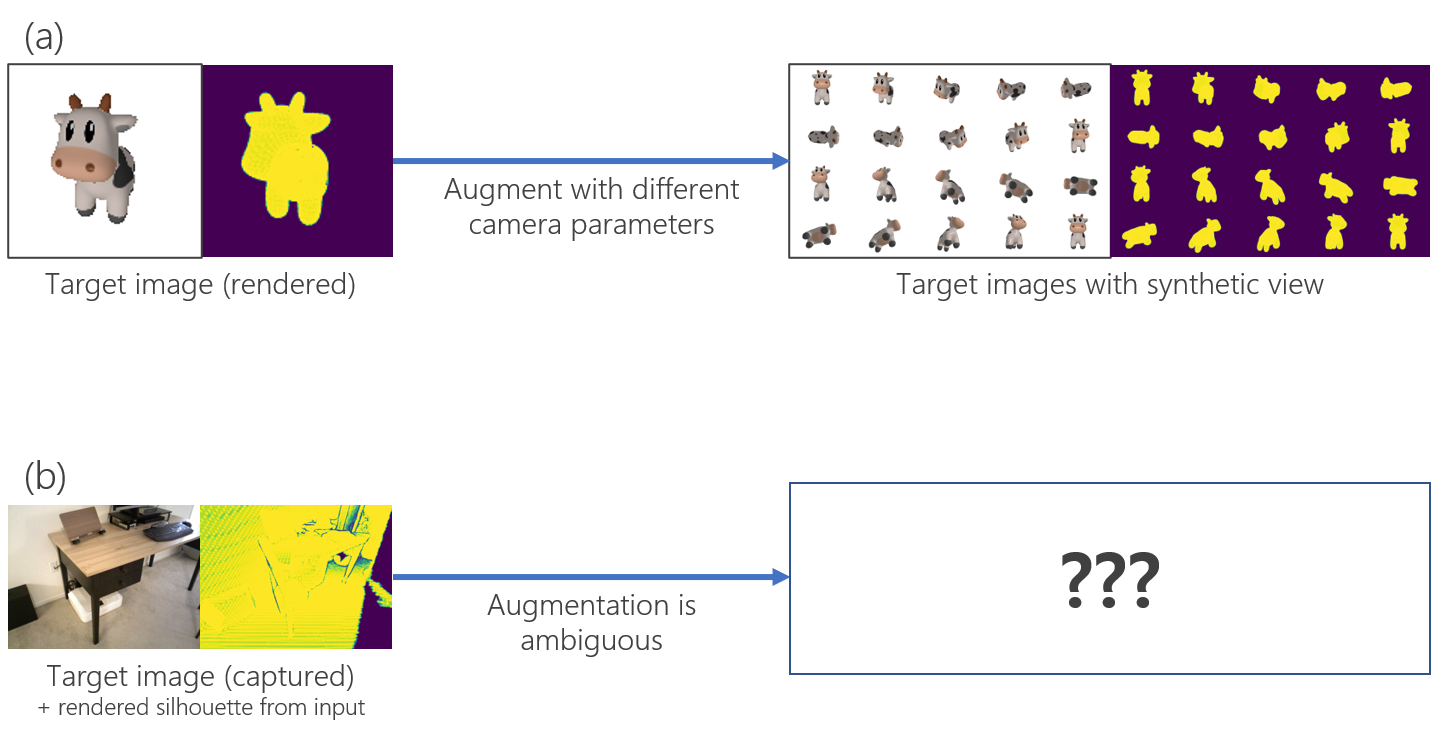
\includegraphics[width=\columnwidth]{figures/2_prev_difference_simple_mesh_and_tsdf_mesh.png}
    \caption{Different setup between optimizing simple mesh and TSDF mesh from SLAM. Previous works aimed to optimize input geometry to set of target images captured with different camera view either synthetically[11][12][13][14] or by taking calibrated real photographs[14]. However, in the case of TSDF mesh from SLAM it is ambiguous since (1) input is not separated with its backgrounds, hence silhouette image is hard to generate (2) we cannot generate synthetic target views (3) it is hard to sample real images from SLAM sequences which captures a region that input mesh represents, since the labeled camera pose paired with target image is estimated value. It is well-known that camera poses from SLAM is inaccurate. (a) It is straightforward to generate synthetic target images if the target image can be rendered. (b) Unlike (a), it is much hard to augment target images in order to optimize indoor TSDF mesh.}
    \label{fig:two}
\end{figure}